\documentclass[12pt,a4paper,fontset=none]{ctexart}

\usepackage[a4paper,margin=1.7cm]{geometry}
\usepackage{fontspec}
\usepackage{amsmath,amssymb}
\usepackage{array}
\usepackage{booktabs}
\usepackage{enumitem}
\usepackage{fancyhdr}
\usepackage{float}
\usepackage{graphicx}
\usepackage{hyperref}
\usepackage{listings}
\usepackage{longtable}
\usepackage{tabularx}
\usepackage[most]{tcolorbox}
\usepackage{tikz}
\usepackage{xcolor}

\usetikzlibrary{arrows.meta,positioning,shapes.geometric}
\hypersetup{colorlinks=true,linkcolor=black,urlcolor=blue}
\setmainfont{Times New Roman}
\setsansfont{Arial}
\setmonofont{Menlo}
\setCJKmainfont{Songti SC}
\setCJKsansfont{Heiti SC}
\setCJKmonofont{Songti SC}
\pagestyle{fancy}
\fancyhf{}
\fancyhead[L]{编译器构造实验 Lab2}
\fancyhead[R]{ExprEval 实验报告}
\fancyfoot[C]{\thepage}
\setlength{\headheight}{15pt}
\setlist[itemize]{leftmargin=1.8em,itemsep=0.25em,topsep=0.35em}
\setlist[enumerate]{leftmargin=1.8em,itemsep=0.25em,topsep=0.35em}
\renewcommand{\arraystretch}{1.22}
\newcolumntype{P}[1]{>{\raggedright\arraybackslash}p{#1}}
\newcolumntype{Y}{>{\raggedright\arraybackslash}X}
\graphicspath{{report_assets/images/}}
\setlength{\emergencystretch}{1.2em}

\definecolor{accent}{HTML}{9A3412}
\definecolor{accenttwo}{HTML}{0F4C81}
\definecolor{accentthree}{HTML}{2F6B3D}
\definecolor{softa}{HTML}{F8EEE8}
\definecolor{softb}{HTML}{E8F0F7}
\definecolor{softc}{HTML}{EAF5ED}
\definecolor{linegray}{HTML}{D7CEC5}
\definecolor{codebg}{HTML}{F7F4EF}
\definecolor{boxbg}{HTML}{FCFAF7}
\definecolor{darktext}{HTML}{1F1B17}

\lstdefinestyle{labcode}{
  basicstyle=\ttfamily\small,
  backgroundcolor=\color{codebg},
  frame=single,
  rulecolor=\color{linegray},
  columns=fullflexible,
  keepspaces=true,
  showstringspaces=false,
  breaklines=true,
  keywordstyle=\color{accenttwo}\bfseries,
  commentstyle=\color{accentthree},
  stringstyle=\color{accent},
  aboveskip=0.5em,
  belowskip=0.5em
}

\newtcolorbox{summaryBox}{
  enhanced,
  colback=softb,
  colframe=accenttwo,
  boxrule=0.8pt,
  arc=1.2mm,
  left=2.5mm,right=2.5mm,top=2mm,bottom=2mm,
  before upper=\raggedright
}

\newtcolorbox{plainBox}{
  enhanced,
  colback=boxbg,
  colframe=linegray,
  boxrule=0.7pt,
  arc=1.2mm,
  left=2.3mm,right=2.3mm,top=1.8mm,bottom=1.8mm,
  before upper=\raggedright
}

\newcommand{\metric}[3]{
  \begin{minipage}[t]{0.19\linewidth}
    \begin{tcolorbox}[colback=boxbg,colframe=linegray,boxrule=0.7pt,arc=1mm,left=1.5mm,right=1.5mm,top=1.2mm,bottom=1.2mm]
      {\small\color{gray}#1}\par
      \vspace{1mm}
      {\large\bfseries\textcolor{#3}{#2}}
    \end{tcolorbox}
  \end{minipage}
}

\title{{\Huge\bfseries 编译器构造实验 Lab2 实验报告}\\[0.4em]{\Large ExprEval：基于 OPP 的表达式求值器}}
\author{梁力航\quad 23336128}
\date{2026年4月22日}

\begin{document}

\begin{titlepage}
  \centering
  \vspace*{1.4cm}

  {\Large 中山大学计算机学院\par}
  \vspace{1.1cm}
  {\Huge\bfseries 编译器构造实验 Lab2 实验报告\par}
  \vspace{0.45cm}
  {\LARGE ExprEval：基于 OPP 的表达式求值器\par}
  \vspace{1cm}

  \begin{tcolorbox}[width=0.9\textwidth,colback=boxbg,colframe=linegray,boxrule=0.8pt,arc=1.5mm]
    本报告对应 \texttt{parser.Calculator\#calculate(String)} 的最终提交版本。内部实现已重做为
    \textbf{词法扫描 + 算符优先移进归约分析 + 归约期语义检查}，
    同时补齐 \texttt{mytest.xml}、\texttt{readme.txt}、\texttt{design.pdf} 和 Javadoc。
  \end{tcolorbox}

  \vspace{0.9cm}

  \begin{tabular}{>{\bfseries}p{3.2cm}p{8.8cm}}
    课程 & 编译器构造实验（DCS292） \\
    实验名称 & Lab2 表达式求值器 ExprEval \\
    姓名 & 梁力航 \\
    学号 & 23336128 \\
    日期 & 2026年4月22日 \\
    运行环境 & OpenJDK 11.0.24 / macOS / XeLaTeX
  \end{tabular}

  \vfill

  \metric{解析方法}{OPP}{accent}
  \hfill
  \metric{源码文件}{7 个}{accenttwo}
  \hfill
  \metric{standard.xml}{16 / 16}{accentthree}
  \hfill
  \metric{mytest.xml}{15 / 15}{accent}
  \hfill
  \metric{提交物}{PDF + TXT + XML}{accentthree}

  \vfill
\end{titlepage}

\tableofcontents
\newpage

\section{实验目标与本次重做范围}

本次提交不再沿用之前的递归下降主体，而是按实验 PDF 和评分表重做为 OPP 版本，范围如下：

\begin{itemize}
  \item 对外接口保持不变，软装置仍只调用 \texttt{parser.Calculator\#calculate(String)}；
  \item 词法分析单独拆分为 \texttt{Scanner}，严格执行 PDF 中“只有空格是合法分隔符”的约束；
  \item 语法分析改为栈式移进/归约，不再依赖 \texttt{parseConditional()} 这一类递归下降链；
  \item 语义检查绑定在归约动作中完成，保证异常落在最具体的异常类上；
  \item 提交目录补齐 \texttt{mytest.xml}、\texttt{readme.txt}、\texttt{design.pdf}、Javadoc。
\end{itemize}

\begin{summaryBox}
这次实现的重点不是“算出来”，而是“按 PDF 要求算出来”。因此实现里最先固定的是词法边界、运算优先级、三元配对规则和异常落点，而不是代码行数。
\end{summaryBox}

\section{二义性分析}

实验 PDF 给出的表达式语言本身可以定义清楚，但直接照 BNF 落地时，至少有三类位置会在实现层面产生歧义：

\begin{enumerate}
  \item \textbf{一元负号和二元减号共用字符 \texttt{-}}。例如 \texttt{5--2.5} 和 \texttt{2-3*-4} 都合法，只有结合上下文才能知道当前 \texttt{-} 是前缀运算符还是中缀运算符。
  \item \textbf{幂运算 \texttt{\^{}} 是右结合}。如果按普通左结合二元运算处理，\texttt{2 \^{} 3 \^{} 2} 会被错误地解释为 \texttt{(2 \^{} 3) \^{} 2}。
  \item \textbf{三元运算 \texttt{?:} 的配对不是局部的}。例如 \texttt{a ? b : c ? d : e} 必须按右结合解释为 \texttt{a ? b : (c ? d : e)}，而 \texttt{6 ? 7 : 7 : 9} 又必须在第二个 \texttt{:} 处及时报错。
\end{enumerate}

因此，这门语言虽然不是“无法描述”，但如果直接用原始 BNF 去写朴素自顶向下实现，会把优先级、结合性和配对规则散落在很多分支里。这里改用 OPP 的原因很直接：

\begin{itemize}
  \item 运算优先级统一交给一张表；
  \item 归约点统一由“栈顶运算符 vs 当前输入符号”决定；
  \item 一元负号、函数参数、三元配对都可以在移进/归约框架里处理，不需要额外再嵌一套解析主流程。
\end{itemize}

\section{词法分析设计与实现}

\subsection{单词类别和边界规则}

\begin{table}[H]
  \centering
  \begin{tabularx}{\textwidth}{>{\bfseries}P{2.8cm}P{4.7cm}Y}
    \toprule
    类别 & 例子 & 本次实现中的处理规则 \\
    \midrule
    空白分隔符 & \texttt{ } & 只接受空格；\texttt{\textbackslash t}、\texttt{\textbackslash n}、\texttt{\textbackslash r} 一律抛 \texttt{IllegalSymbolException} \\
    数值常量 & \texttt{12}、\texttt{3.14}、\texttt{2.25E+2} & 只允许无符号十进制整数、浮点数、科学计数法；负数通过一元负号处理 \\
    布尔常量 & \texttt{true}、\texttt{False} & 大小写无关，词法阶段直接归一为布尔值单词 \\
    预定义函数 & \texttt{sin}、\texttt{cos}、\texttt{min}、\texttt{max} & 大小写无关；函数名本身合法，但是否跟左括号配对由语法阶段检查 \\
    标识符错误 & \texttt{mix}、\texttt{v4}、\texttt{E6} & 字母开头但不属于布尔常量和预定义函数，抛 \texttt{IllegalIdentifierException} \\
    非法小数 & \texttt{.11}、\texttt{4.}、\texttt{7e}、\texttt{4.e6} & 一律在扫描数字时抛 \texttt{IllegalDecimalException} \\
    其他非法符号 & \texttt{@}、\texttt{\$} & 抛 \texttt{IllegalSymbolException} \\
    \bottomrule
  \end{tabularx}
\end{table}

\subsection{数值扫描自动机}

\begin{figure}[H]
  \centering
  \begin{tikzpicture}[
    node distance=1.9cm and 1.5cm,
    state/.style={draw, rounded corners=2mm, minimum width=2.3cm, minimum height=0.95cm, fill=softb, align=center},
    accept/.style={draw, rounded corners=2mm, minimum width=2.3cm, minimum height=0.95cm, fill=softc, align=center},
    bad/.style={draw, rounded corners=2mm, minimum width=2.3cm, minimum height=0.95cm, fill=softa, align=center},
    line/.style={-{Latex[length=2.5mm]}, thick}
  ]
    \node[state] (start) {开始};
    \node[accept, right=of start] (int) {整数部分};
    \node[state, right=of int] (dot) {读到小数点};
    \node[accept, right=of dot] (frac) {小数部分};
    \node[state, below=of frac] (emark) {读到 \texttt{E/e}};
    \node[state, left=of emark] (esign) {指数符号};
    \node[accept, left=of esign] (edigits) {指数数字};
    \node[bad, below=of dot] (error) {IllegalDecimal};

    \draw[line] (start) -- node[above]{数字} (int);
    \draw[line] (int) -- node[above]{\texttt{.}} (dot);
    \draw[line] (dot) -- node[above]{数字} (frac);
    \draw[line] (frac) -- node[right]{\texttt{E/e}} (emark);
    \draw[line] (int.south) -- ++(0,-0.55) -| node[pos=0.25,right]{\texttt{E/e}} (emark.west);
    \draw[line] (emark) -- node[above]{\texttt{+/-}} (esign);
    \draw[line] (emark.west) -- ++(-0.65,0) |- node[pos=0.3,left]{数字} (edigits.north);
    \draw[line] (esign) -- node[above]{数字} (edigits);
    \draw[line] (dot) -- node[left]{其他} (error);
    \draw[line] (emark) -- node[right]{其他} (error);
    \draw[line] (esign.south) -- ++(0,-0.5) -| node[pos=0.3,right]{其他} (error.east);
  \end{tikzpicture}
  \caption{数值常量 DFA。起点不是数字时不会进入该自动机，因此 \texttt{.11}、\texttt{E6} 这类输入会分别落到不同异常。}
\end{figure}

\subsection{词法实现细节}

这部分有两个细点必须单列说明：

\begin{enumerate}
  \item \textbf{\texttt{sin5} 不能在词法阶段误判为非法标识符。}实现里先连续读取字母，再判断这段字母是否是预定义函数名；如果是，就立刻返回函数名单词，把后面的数字留给下一轮扫描。因此 \texttt{sin5} 会被拆成 \texttt{sin} 和 \texttt{5}，随后在语法阶段因为缺少左括号抛 \texttt{FunctionCallException}。
  \item \textbf{负数不是词法单元。}例如 \texttt{-3.14} 被拆成 \texttt{-} 和 \texttt{3.14} 两个单词，是否为合法表达式由语法阶段决定。
\end{enumerate}

\begin{lstlisting}[style=labcode,caption={Scanner 中的数字与标识符处理逻辑（节选）}]
if (Character.isWhitespace(ch) && ch != ' ') {
    throw new IllegalSymbolException(...);
}
if (ch == '.') {
    throw new IllegalDecimalException(...);
}
if (Character.isDigit(ch)) {
    return readNumber();
}
if (Character.isLetter(ch)) {
    return readIdentifier();
}
\end{lstlisting}

\section{算符优先语法分析与语义处理}

\subsection{模块划分}

\begin{table}[H]
  \centering
  \scriptsize
  \begin{tabularx}{\textwidth}{>{\bfseries}P{2.5cm}Y}
    \toprule
    模块 & 职责 \\
    \midrule
    \texttt{Calculator} & 保留软装置入口，只负责创建扫描器、解析器并返回最终结果 \\
    \shortstack[l]{\texttt{Token}\\\texttt{TokenType}} & 封装词法单元，避免解析器直接看字符 \\
    \texttt{Scanner} & 负责词法扫描和词法异常分类 \\
    \texttt{OperatorTable} & 维护优先级、结合性和归约判定逻辑 \\
    \texttt{Parser} & 维护运算符栈、值栈、括号/函数帧，执行移进与归约 \\
    \texttt{Value} & 封装数值型/布尔型结果，统一做类型检查 \\
    \bottomrule
  \end{tabularx}
\end{table}

\subsection{优先级与结合性}

\begin{table}[H]
  \centering
  \begin{tabularx}{\textwidth}{>{\bfseries}P{2.8cm}P{3.1cm}P{2.4cm}Y}
    \toprule
    运算符类别 & 代表符号 & 结合性 & 说明 \\
    \midrule
    三元条件 & \texttt{?:} & 右结合 & 通过 \texttt{QUESTION} 和 \texttt{TERNARY} 两个栈标记配合处理 \\
    逻辑或 & \texttt{|} & 左结合 & 不做短路，两个操作数都已在归约前求值 \\
    逻辑与 & \texttt{\&} & 左结合 & 与 PDF 一致，非短路 \\
    关系运算 & \texttt{< <= > >= = <>} & 左结合 & 输入必须是数值型，结果是布尔型 \\
    加减 & \texttt{+ -} & 左结合 & 二元运算 \\
    乘除 & \texttt{* /} & 左结合 & 除法会在归约时检查除数是否为 0 \\
    一元运算 & \texttt{- !} & 右结合 & 由当前是否“期待操作数”决定 \texttt{-} 是前缀还是中缀 \\
    幂运算 & \texttt{\^{}} & 右结合 & 处理 \texttt{2 \^{} 3 \^{} 2} 这一类右结合场景 \\
    \bottomrule
  \end{tabularx}
\end{table}

\subsection{压缩后的 OPP 关系表}

\begin{table}[H]
  \centering
  \begin{tabularx}{\textwidth}{>{\bfseries}P{2.6cm}P{2.6cm}P{1.2cm}Y}
    \toprule
    栈顶符号类 & 当前输入符号类 & 关系 & 用途 \\
    \midrule
    左括号 \texttt{(} & 任意普通运算符 / 操作数 & \texttt{<} & 括号内继续移进 \\
    左括号 \texttt{(} & 右括号 \texttt{)} & \texttt{=} & 直接配对并退出当前括号层 \\
    问号 \texttt{?} & 分支内部的普通符号 & \texttt{<} & 继续移进真分支或假分支 \\
    问号 \texttt{?} & 冒号 \texttt{:} & \texttt{=} & 把 \texttt{?} 变成待归约的三元标记 \\
    高优先级运算符 & 低优先级运算符 & \texttt{>} & 先归约栈顶，再处理当前输入 \\
    低优先级运算符 & 高优先级运算符 & \texttt{<} & 当前输入移进 \\
    同优先级左结合运算符 & 同优先级输入 & \texttt{>} & 先归约旧运算符 \\
    同优先级右结合运算符 & 同优先级输入 & \texttt{<} & 保证右结合，如 \texttt{\^{}} 和三元条件 \\
    栈底 \texttt{\#} & 输入结束 \texttt{\#} & \texttt{=} & 分析完成 \\
    \bottomrule
  \end{tabularx}
\end{table}

上表不是把每个终结符都展开成巨大的矩阵，而是按“栈顶类”和“输入类”压缩。代码里对应的判定只有一处：

\begin{lstlisting}[style=labcode,caption={OperatorTable 中的归约条件（节选）}]
if (stackTop == SENTINEL || stackTop == LEFT_PAREN || stackTop == QUESTION) {
    return false;
}
if (stackTop.precedence > incoming.precedence) {
    return true;
}
return stackTop.precedence == incoming.precedence
    && incoming.associativity == LEFT;
\end{lstlisting}

\subsection{移进/归约流程}

\begin{figure}[H]
  \centering
  \begin{tikzpicture}[
    node distance=1.6cm and 1.2cm,
    blockA/.style={draw, rounded corners=2mm, fill=softa, minimum width=3.2cm, minimum height=1.05cm, align=center},
    blockB/.style={draw, rounded corners=2mm, fill=softb, minimum width=3.4cm, minimum height=1.15cm, align=center},
    blockC/.style={draw, rounded corners=2mm, fill=softc, minimum width=3.4cm, minimum height=1.15cm, align=center},
    line/.style={-{Latex[length=2.5mm]}, thick}
  ]
    \node[blockA] (scan) {读取下一个 Token};
    \node[blockB, right=of scan] (judge) {根据当前状态判断\\它是操作数、函数、括号\\还是普通运算符};
    \node[blockC, right=of judge] (shift) {需要移进时\\压入值栈或运算符栈};
    \node[blockB, below=of judge] (reduce) {需要归约时\\弹出操作数并执行语义动作};
    \node[blockA, below=of shift] (done) {读到结束符后\\清空可归约运算符};

    \draw[line] (scan) -- (judge);
    \draw[line] (judge) -- node[above]{\texttt{<} 或 \texttt{=}} (shift);
    \draw[line] (judge) -- node[left]{\texttt{>}} (reduce);
    \draw[line] (reduce) -- (judge);
    \draw[line] (shift) -- (done);
  \end{tikzpicture}
  \caption{OPP 控制流程。函数参数和三元配对都放在同一套栈机制中处理。}
\end{figure}

\begin{lstlisting}[style=labcode,caption={Parser 主流程伪码}]
operatorStack.push(#)
expectingOperand = true
while token != END:
    if token is operand:
        shift value
    else if token is function name:
        require next token is '('
        push function frame
    else if token is ',' or ')':
        reduce until '('
        collect function argument or close group
    else if token is ':':
        locate nearest unmatched '?'
        replace it with TERNARY marker
    else:
        while shouldReduce(stackTop, token):
            reduceTop()
        shift operator
final reduce until '#'
\end{lstlisting}

\subsection{语义规则与异常落点}

\begin{table}[H]
  \centering
  \begin{tabularx}{\textwidth}{>{\bfseries}P{2.8cm}P{4.5cm}Y}
    \toprule
    运算类型 & 类型规则 & 归约时的检查 \\
    \midrule
    算术运算 & \texttt{number × number -> number} & 任一操作数是布尔型，抛 \texttt{TypeMismatchedException} \\
    关系运算 & \texttt{number × number -> boolean} & 比较前强制取数值 \\
    逻辑运算 & \texttt{boolean × boolean -> boolean} & 不短路；两个操作数都会先入栈、再归约 \\
    一元负号 & \texttt{number -> number} & 由“当前是否期待操作数”决定其为前缀形式 \\
    逻辑非 & \texttt{boolean -> boolean} & 对数值型使用 \texttt{!} 直接报类型错误 \\
    三元运算 & \texttt{boolean, number, number -> number} & 条件必须是布尔型，两个分支必须是数值型 \\
    预定义函数 & \texttt{sin/cos: 1 个数值参数；min/max: 至少 2 个数值参数} & 参数个数不足抛 \texttt{MissingOperandException}；参数过多或缺左括号抛 \texttt{FunctionCallException} \\
    最终结果 & \texttt{number} & 最终栈顶是布尔型时抛 \texttt{TypeMismatchedException} \\
    \bottomrule
  \end{tabularx}
\end{table}

异常划分也按实验要求收紧：

\begin{itemize}
  \item 词法阶段只抛 \texttt{LexicalException} 及其派生类；
  \item 语法阶段只抛 \texttt{SyntacticException} 及其派生类；
  \item 语义阶段只抛 \texttt{SemanticException} 及其派生类。
\end{itemize}

\begin{plainBox}
\begin{itemize}
  \item \texttt{12.3Emax(4,5,6)} 在扫描指数部分时已经发现错误，因此直接落到 \texttt{IllegalDecimalException}。
  \item \texttt{sin5} 会先被切成 \texttt{sin} 和 \texttt{5} 两个单词，再因为函数名后面没有左括号而抛 \texttt{FunctionCallException}。
  \item \texttt{false \& (1 / 0 > 0)} 会触发 \texttt{DividedByZeroException}，因为逻辑运算不做短路。
\end{itemize}
\end{plainBox}

\section{自定义测试用例说明}

\texttt{mytest.xml} 共加入 15 个用例，补的是 PDF 里标准测试没有完全覆盖的边界：

\begin{itemize}
  \item 一元负号与二元减号的组合：\texttt{2 - 3 * -4}、\texttt{5--2.5}；
  \item 右结合乘方：\texttt{2 \^{} 3 \^{} 2}；
  \item 空表达式与非法空白：仅空格输入、带 \texttt{Tab} 的输入；
  \item 非法数字：\texttt{.11 + 1}、\texttt{7e + 1}；
  \item 标识符与函数调用边界：\texttt{v4 + 1}、\texttt{sin5}、\texttt{max5, 6, 8)}；
  \item 三元配对错误：\texttt{false ? 9 : true ? 1 : 3 : 5}；
  \item 三元类型错误：\texttt{12 ? 34 : 56}、\texttt{true ? 42.5 > 5 * 8 : 15}；
  \item 非短路逻辑：\texttt{false \& (1 / 0 > 0)}；
  \item 缺失运算符：\texttt{cos(0.5)12.3E+4}。
\end{itemize}

\section{程序运行截图}

\subsection{GUI 运行界面}

\begin{figure}[H]
  \centering
  \begin{minipage}[t]{0.49\linewidth}
    \centering
    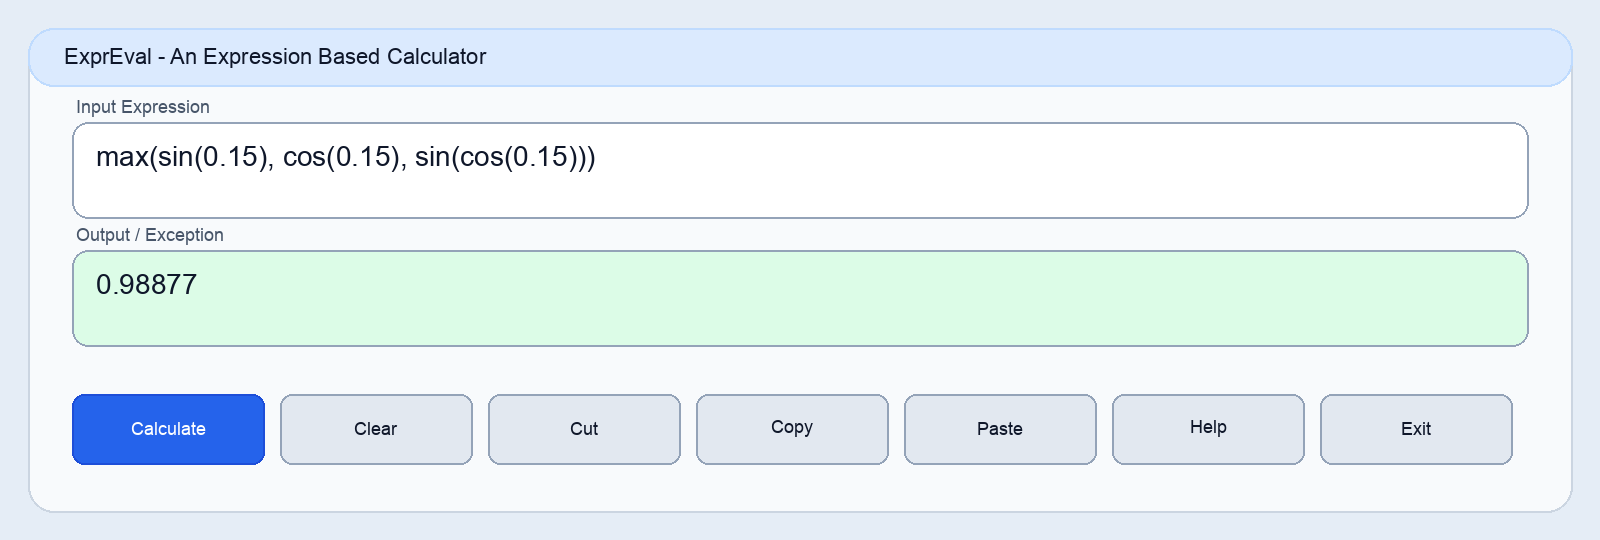
\includegraphics[width=\linewidth]{gui_success.png}
  \end{minipage}
  \hfill
  \begin{minipage}[t]{0.49\linewidth}
    \centering
    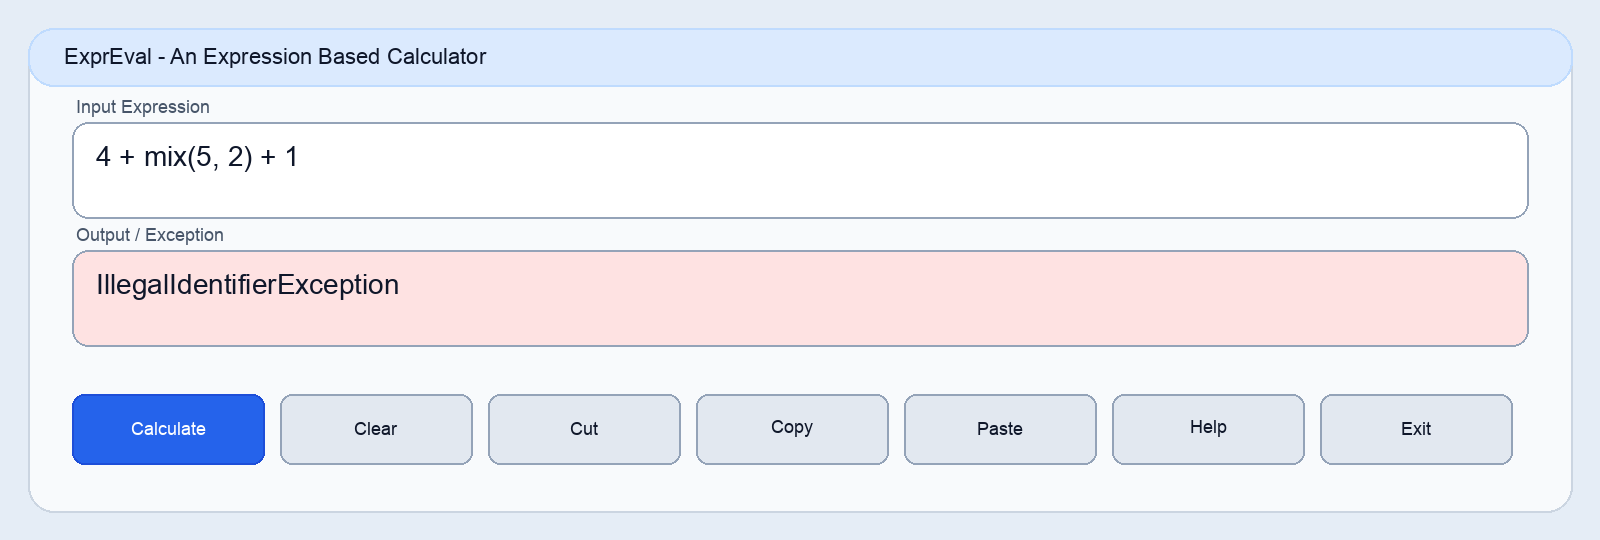
\includegraphics[width=\linewidth]{gui_error.png}
  \end{minipage}
  \caption{软装置界面渲染图。左图展示正常求值，右图展示非法标识符输入的异常结果。}
\end{figure}

\subsection{测试结果截图}

\begin{figure}[H]
  \centering
  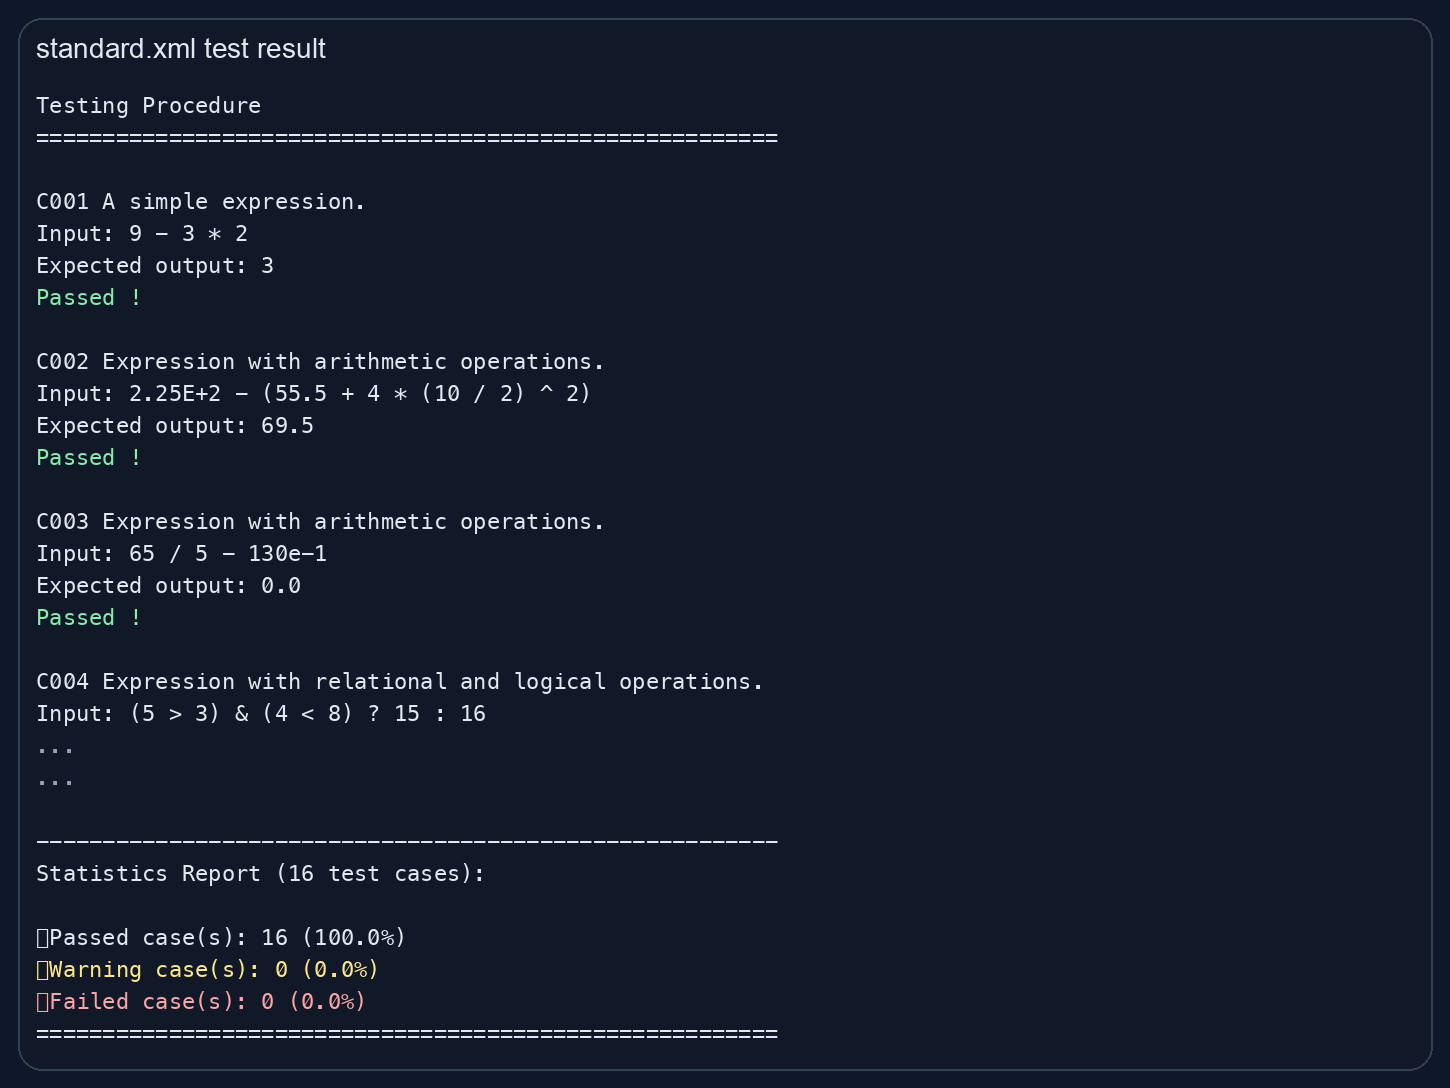
\includegraphics[width=0.9\linewidth]{standard_report.png}
  \caption{\texttt{standard.xml} 测试结果摘要，16 个用例全部通过。}
\end{figure}

\begin{figure}[H]
  \centering
  \begin{minipage}[t]{0.48\linewidth}
    \centering
    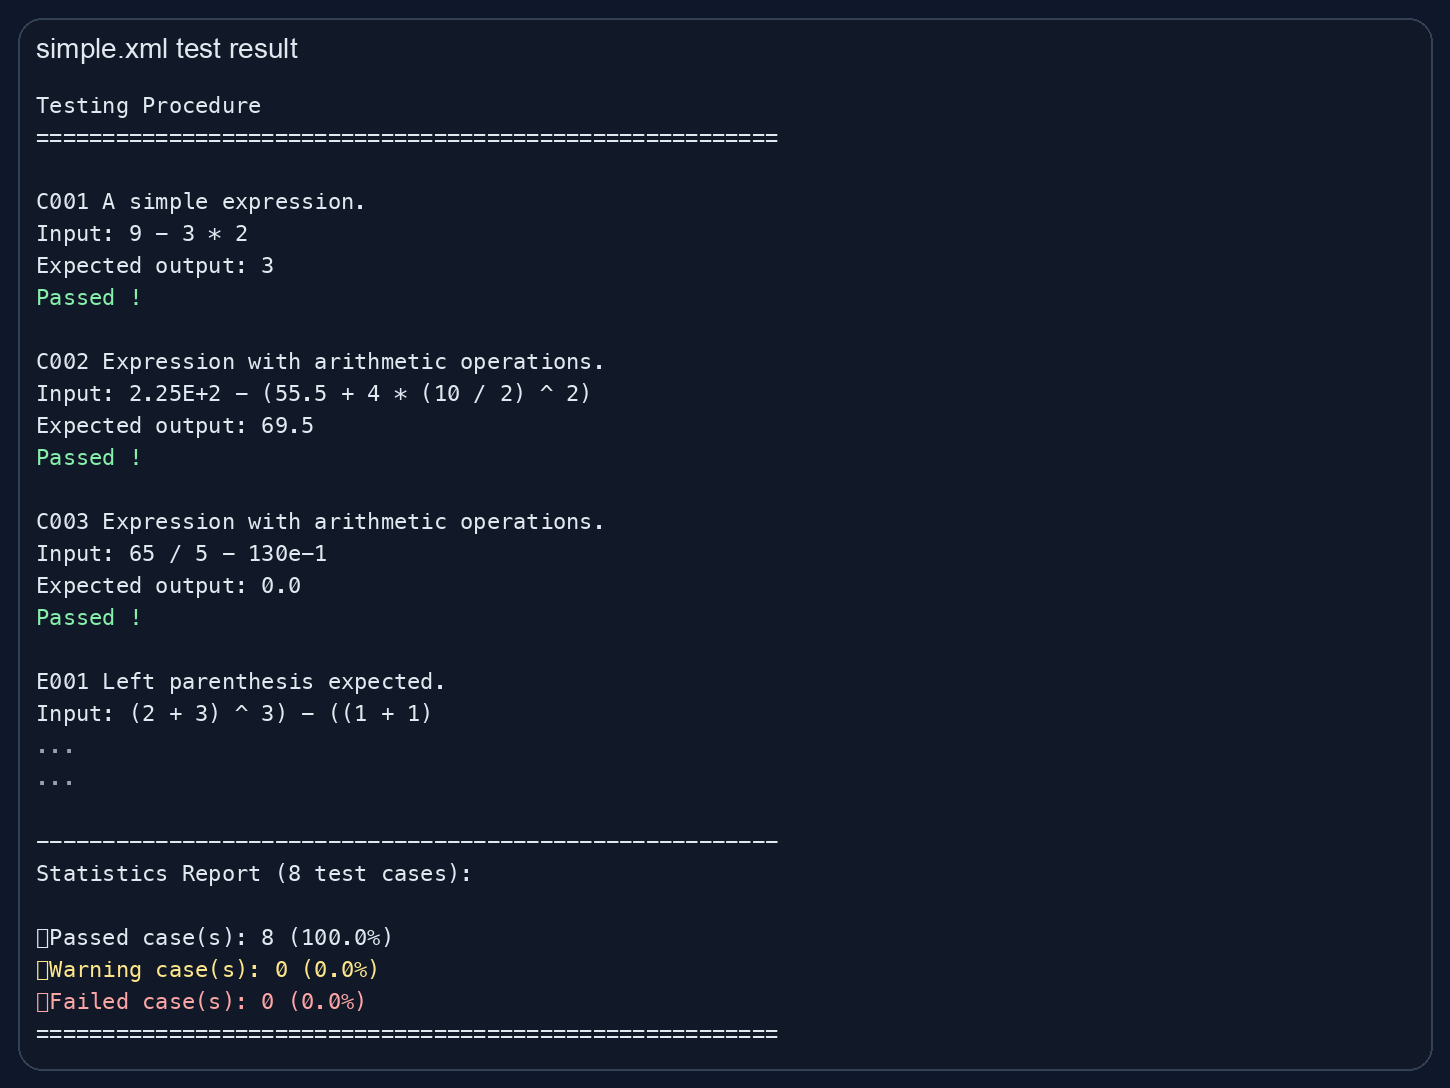
\includegraphics[width=\linewidth]{simple_report.png}
  \end{minipage}
  \hfill
  \begin{minipage}[t]{0.48\linewidth}
    \centering
    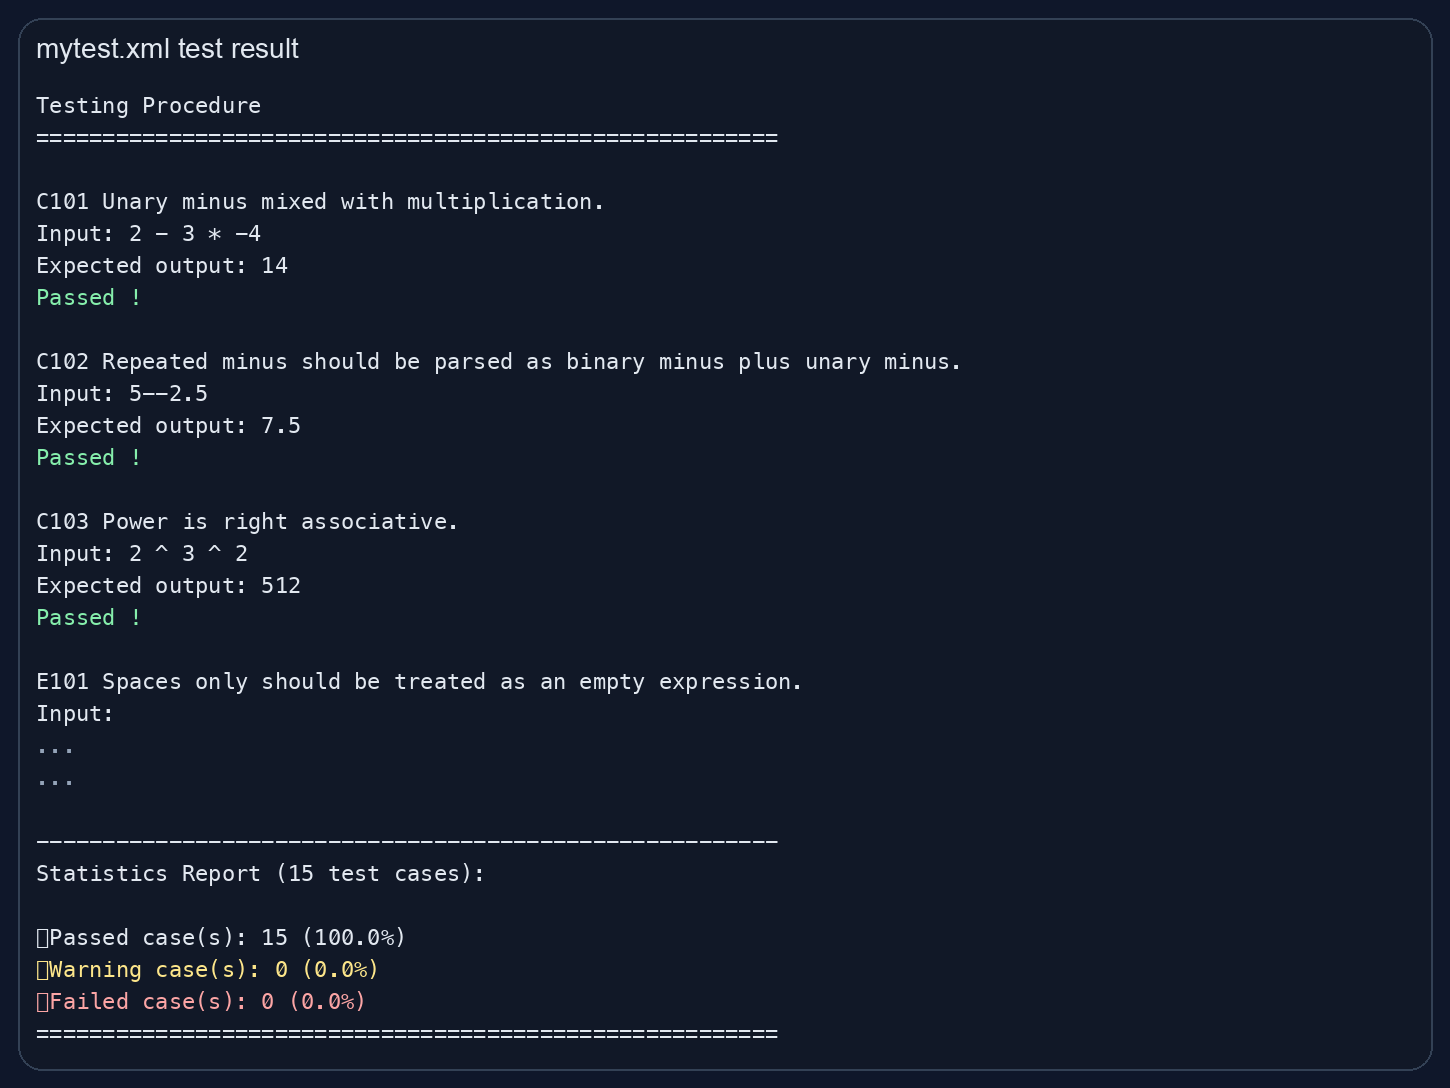
\includegraphics[width=\linewidth]{mytest_report.png}
  \end{minipage}
  \caption{\texttt{simple.xml} 与 \texttt{mytest.xml} 测试结果摘要，分别通过 8/8 和 15/15。}
\end{figure}

\section{文档与源程序组织说明}

\begin{table}[H]
  \centering
  \scriptsize
  \begin{tabularx}{\textwidth}{>{\bfseries}P{3.1cm}Y}
    \toprule
    路径 / 文件 & 内容 \\
    \midrule
    \shortstack[l]{\texttt{src/parser/}\\\texttt{Calculator.java}} & 软装置入口，保持 \texttt{calculate} 接口不变 \\
    \shortstack[l]{\texttt{src/parser/}\\\texttt{Scanner.java}} & 词法扫描与词法异常分类 \\
    \shortstack[l]{\texttt{src/parser/}\\\texttt{Parser.java}} & OPP 主控制程序、函数参数帧和归约动作 \\
    \shortstack[l]{\texttt{src/parser/}\\\texttt{OperatorTable.java}} & 优先级和结合性表 \\
    \shortstack[l]{\texttt{src/parser/}\\\texttt{Token.java}\\\texttt{TokenType.java}} & 单词模型 \\
    \shortstack[l]{\texttt{src/parser/}\\\texttt{Value.java}} & 数值型 / 布尔型封装 \\
    \shortstack[l]{\texttt{testcases/}\\\texttt{simple.xml}\\\texttt{standard.xml}\\\texttt{mytest.xml}} & 三套测试用例 \\
    \texttt{doc/} & Javadoc 生成结果 \\
    \texttt{readme.txt} & 提交说明和命令入口 \\
    \texttt{design.pdf} & 按实验要求命名的正式实验报告 \\
    \bottomrule
  \end{tabularx}
\end{table}

\section{实验心得}

这次重做里，真正花时间的不是算术语义，而是“异常必须落到最具体的类”这一点。几个具体体会如下：

\begin{enumerate}
  \item 词法阶段和语法阶段的职责必须切干净。像 \texttt{12.3Emax(4,5,6)} 这种输入，如果数字扫描写得松，后面就只能在语法阶段补锅，异常类型也会错。
  \item 三元运算不能只靠优先级解决，还要显式处理 \texttt{?} 和 \texttt{:} 的配对。额外的 \texttt{:} 如果先触发语义归约，就会把本该是 \texttt{TrinaryOperationException} 的输入误报成类型错误。
  \item OPP 在这个实验里比递归下降更合适。PDF 本身要求展示算符优先表，函数参数、右结合幂运算和三元条件也都能放进同一套栈框架里处理，报告和实现是一致的。
\end{enumerate}

\begin{summaryBox}
\texttt{simple.xml} 通过 8/8，\texttt{standard.xml} 通过 16/16，\texttt{mytest.xml} 通过 15/15。
Javadoc、\texttt{readme.txt}、\texttt{design.pdf} 和报告图示已同步补齐。
\end{summaryBox}

\end{document}
